\section{引言}

空气质量预测是环境科学研究中的重要课题,对于环境保护和公共健康具有重要意义\cite{zhang2020air}。随着工业化和城市化的快速发展,空气污染问题日益突出,准确预测空气质量变化趋势成为当前研究的热点问题。近年来,随着数据采集技术的进步和计算能力的提升,基于机器学习的预测方法在空气质量预测领域展现出巨大潜力\cite{kim2019hybrid}。相比传统的统计方法,机器学习方法能够更好地处理非线性关系,并且可以综合考虑多个影响因素。

准确的空气质量预测具有多方面的实际应用价值。首先,它可以为环境保护部门提供决策支持,帮助制定更有针对性的污染防治措施;其次,可以帮助公众及时了解空气质量状况,做好个人防护准备;再次,对于城市规划和环境治理,精确的预测可以提供科学依据,促进环境污染治理的精准化和科学化。本研究的主要目标是构建准确的空气质量预测模型,分析影响空气质量的关键因素,评估不同机器学习算法的预测性能,并提供可实施的预警方案建议。

本研究采用了系统的研究方法,如图\ref{fig:workflow}所示。首先对原始数据进行预处理,包括缺失值处理、异常值检测和特征工程等步骤;然后构建多个机器学习模型,包括随机森林、决策树、支持向量机和神经网络等;最后通过交叉验证和多个评估指标对模型性能进行全面评估。研究结果不仅展示了不同模型的预测效果,还揭示了各个气象因素对空气质量的影响程度。

\begin{figure}[H]
    \centering
    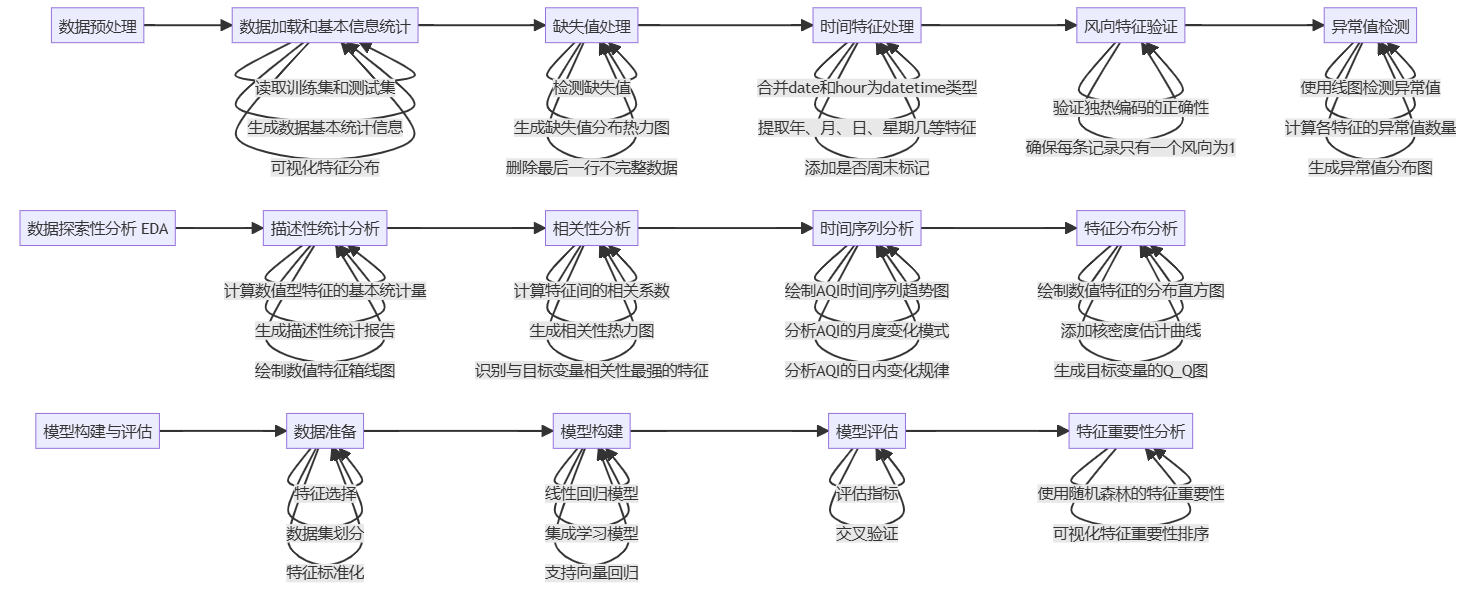
\includegraphics[width=0.8\textwidth]{images/export.png}
    \caption{研究工作流程图}
    \label{fig:workflow}
\end{figure} 